\documentclass[xcolor=dvipsnames,10pt,aspectratio=169]{beamer}
%\documentclass[xcolor=dvipsnames,10pt]{beamer}
\usepackage{etex}
\usepackage{pgf,pgfarrows,pgfnodes,pgfautomata,pgfheaps,pgfshade}
\usepackage[absolute,overlay]{textpos} 
%\usepackage{algorithm}
\usepackage{amsmath,amssymb}
\usepackage[utf8]{inputenc} 
\usepackage{colortbl}
\usepackage{graphicx} 
\usepackage[english]{babel}
\usepackage{tabularx} 
\usepackage{multirow}
\usepackage{booktabs}
\usepackage{listings}
%\usepackage{multimedia}
\usepackage{animate}
\usepackage{xcolor}
\usepackage{array}
\usepackage{longtable}
\usepackage{makecell}
\usepackage{caption}
\usetheme{Madrid} 
\usepackage{amsmath}
\usepackage{movie15}
\usepackage{tikz}
\usetikzlibrary{shapes.geometric,arrows,shadows}

\lstset{ %
%	backgroundcolor=\color{white},   % choose the background color; you must add \usepackage{color} or \usepackage{xcolor}
%	basicstyle=\footnotesize,        % the size of the fonts that are used for the code
	basicstyle=\scriptsize,        % the size of the fonts that are used for the code
	breakatwhitespace=false,         % sets if automatic breaks should only happen at whitespace
	breaklines=true,                 % sets automatic line breaking
	captionpos=t,                    % sets the caption-position to bottom
	commentstyle=\color{mygreen},    % comment style
	deletekeywords={...},            % if you want to delete keywords from the given language
	escapeinside={\%*}{*)},          % if you want to add LaTeX within your code
	extendedchars=true,              % lets you use non-ASCII characters; for 8-bits encodings only, does not work with UTF-8
%	frame=single,                    % adds a frame around the code
	keepspaces=true,                 % keeps spaces in text, useful for keeping indentation of code (possibly needs columns=flexible)
	keywordstyle=\color{blue},       % keyword style
%	language=make,                 % the language of the code
	morekeywords={*,...},            % if you want to add more keywords to the set
%	numbers=left,                    % where to put the line-numbers; possible values are (none, left, right)
%	numbersep=5pt,                   % how far the line-numbers are from the code
	numberstyle=\tiny\color{mygray}, % the style that is used for the line-numbers
	rulecolor=\color{black},         % if not set, the frame-color may be changed on line-breaks within not-black text (e.g. comments (green here))
	showspaces=false,                % show spaces everywhere adding particular underscores; it overrides 'showstringspaces'
	showstringspaces=false,          % underline spaces within strings only
	showtabs=false,                  % show tabs within strings adding particular underscores
	stepnumber=2,                    % the step between two line-numbers. If it's 1, each line will be numbered
}

\definecolor{mygreen}{rgb}{0,0.6,0}
\definecolor{mygray}{rgb}{0.5,0.5,0.5}
\definecolor{mymauve}{rgb}{0.58,0,0.82}

\usecolortheme{beaver}
\newcommand{\ul}{\underline}
\setbeamertemplate{footline}{\scriptsize{\vspace*{0.3cm}\hspace*{15cm}\insertframenumber\,/\,\inserttotalframenumber}}
\setbeamertemplate{caption}[numbered]
\setbeamerfont{caption}{size=\fontsize{8}{5}}

\setbeamercolor{block title}{	bg=Sepia , fg = White}
\setbeamercolor{block body}{bg=Brown!15, fg=Sepia }
\setbeamercolor{item projected}{bg=Sepia, fg=White}
\setbeamercolor{number projected}{bg = Black}

%declara as imagens usadas no layout do slide
\pgfdeclareimage[height=0.8cm]{mflab}{figuras/logo_mflab_transparente.png}
\pgfdeclareimage[height=1.0cm]{logoufu}{figuras/logo_ufu.jpg}
\pgfdeclareimage[height=1.0cm]{petro}{figuras/petrobras_2.png}

%posiciona o logotipo do MFLab
\setlength{\TPHorizModule}{1mm}
\setlength{\TPVertModule}{1mm}
\newcommand{\placelogomflab} 
{ 
	\begin{textblock}{13}(150.0,0.0)
		\pgfuseimage{mflab} 
	\end{textblock} 
	
	\begin{textblock}{13}(150.0,70.0)
		\pgfuseimage{petro} 
	\end{textblock} 
}
\setlength{\TPHorizModule}{1mm}
\setlength{\TPVertModule}{1mm}
\newcommand{\placelogo} 
{ 
	\begin{textblock}{13}(150.0,0.0)
		\pgfuseimage{mflab} 
	\end{textblock} 
	
	\begin{textblock}{13}(0.0,80.0)
		\pgfuseimage{petro} 
	\end{textblock} 
}

\title{NEURAL NETWORK ASSISTED CAVITY CONVECTION FLOW}

\author{ Felipe J. O. Ribeiro \\ \and \\ Prof. Dr. Aristeu da Silveira Neto \\ Prof. Dr. Aldemir Aparecido Cavallini Junior}

\date{\tiny{\today}}
\newcolumntype{C}[1]{>{\centering\let\newline\\\arraybackslash\hspace{0pt}}m{#1}}


\begin{document}

\begin{frame}\placelogomflab
	\frametitle 
	{ \vfill
		\centering
		{
		\small{Federal University of Uberlândia}\\
			% \small{Programa de Pós-Graduação em Engenharia Mecânica}\\
		\small{Fluid Mechanics laboratory}\\
		}
	}
	\maketitle
\end{frame}

\section<presentation>*{Index}
	
\begin{frame}
	\frametitle{Index}\placelogomflab 
	{\scriptsize \tableofcontents}
\end{frame}

\AtBeginSection[]
{
 \begin{frame}<beamer>
  \frametitle{Index}\placelogomflab 
  {\scriptsize \tableofcontents[current,currentsection]}
 \end{frame}
}

\AtBeginSubsection[]
{
 \begin{frame}<beamer>
  \frametitle{Index}\placelogomflab 
  {\scriptsize \tableofcontents[current,currentsubsection]}
 \end{frame}
}


\section{Introduction}

\begin{frame}\frametitle{Objectives}
	\centering
	The present text seeks to document the development of this research work with detail. from mathematical and theoretical developments to progress in technical and organizational aspects.
	\vspace{0.5cm}

	\flushleft
	The core topics of this study are:\\
	\quad $\bullet$ Theoretical and mathematical development of two-dimensional cavity flow;\\
	\quad $\bullet$ Development of artificial neural network machine learning in FORTRAN;\\
	\quad $\bullet$ Enhancement of the visualization methods with OpenGL in FORTRAN;\\
	\quad $\bullet$ Development of MPI methodologies.\\
\end{frame}

\begin{frame}\frametitle{Bidimensional convective flow in a cavity}
	\begin{minipage}[h!]{0.39\textwidth}
		$\bullet$ Natural convection is a classic cavity flow phenomenon. it represents many industrial and everyday situations;\\
		$\bullet$ To simulate such a phenomenon a two or three-dimensional domain is necessary. Which brings new challenges compared to the previous poiseuille flow project;\\
		$\bullet$ Despite dealing with fluid mass changes, the flow is considered incompressible, as volumetric changes are negligible;\\

	\end{minipage}
	\begin{minipage}[h!]{0.6\textwidth}
		\begin{figure}[h!]
			\centering
			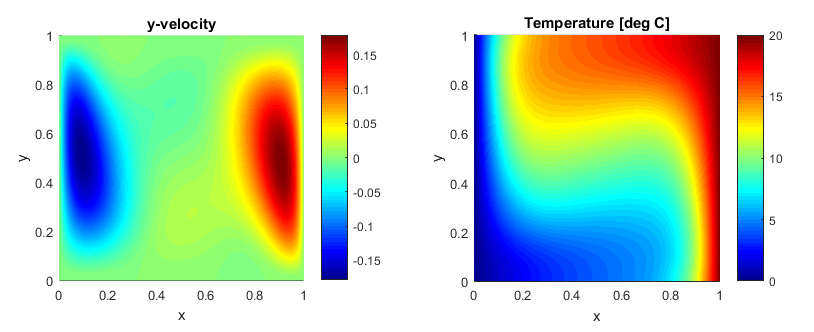
\includegraphics[trim = {0cm 0cm 0cm 0cm}, clip , angle=0, scale=0.45]{./my_images/NaturalConvectionFromNet.png}
			\caption{cavity convection example.}
		\end{figure}
	\end{minipage}
\end{frame}

\begin{frame}\frametitle{Artificial neural networks}
	\begin{minipage}[h!]{0.39\textwidth}
		$\bullet$ They seek to mimetize the biology of brains to emulate it's learning capabilities.\\
		$\bullet$ Its based on the neuron entities and it is defined by the structure of neurons and the weights of each connection.\\
		$\bullet$ Training the network, or, the learning process, as it is called, consistis in determining the weights of each connection based on multiples tests and loss calculation. A gradient descent is used to obtain the weights with which the error is the minimal in a given training set.
	\end{minipage}
	\begin{minipage}[h!]{0.6\textwidth}
		\begin{figure}[h!]
			\centering
			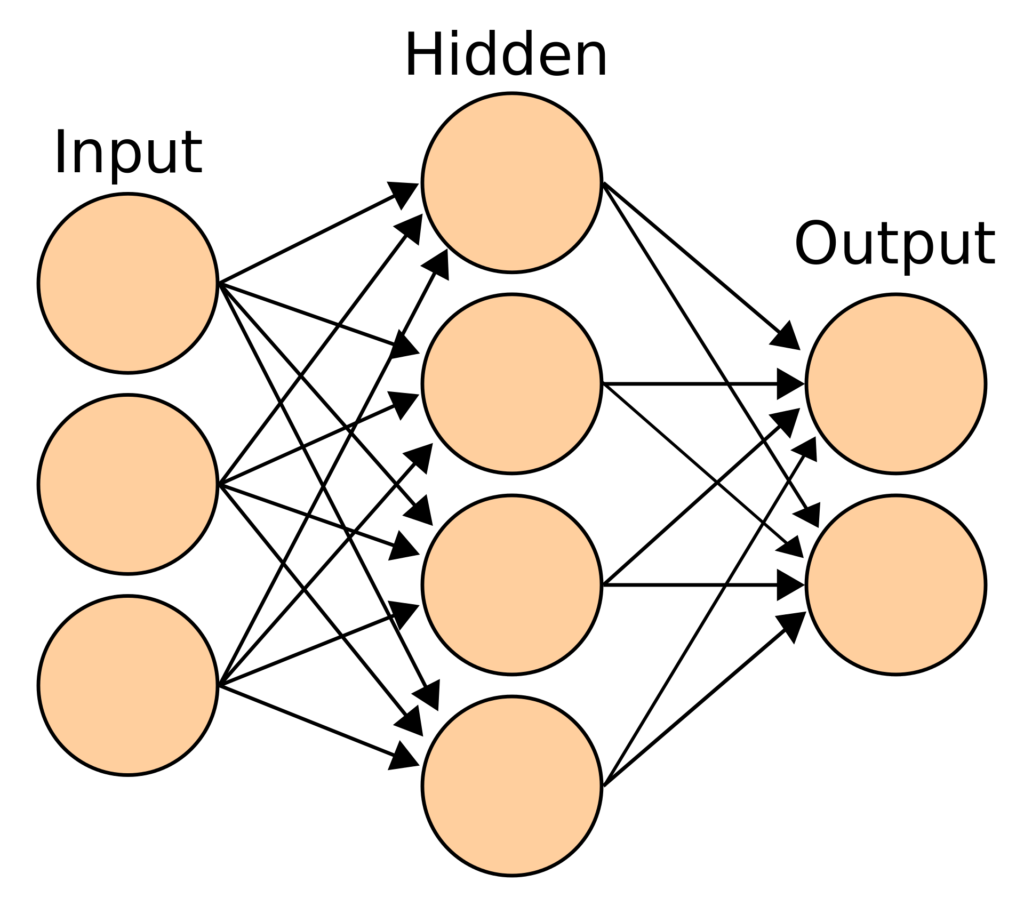
\includegraphics[trim = {0cm 0cm 0cm 0cm}, clip , angle=0, scale=0.18]{./my_images/neural_figure.png}
			\caption{Simple neural network. Basic perceptrons structure.}
		\end{figure}
	\end{minipage}
\end{frame}


\begin{frame}\frametitle{Bibliography}
	$\bullet$ Fourier Neural Operator for Parametric Partial Differential Equations. (Zongyi L., Nikola K., Kamyar A., Burigede L., Kaushik B. Andrew S. Anima A.)\\

	\vspace{0.5cm}

	Same authors:\\
	$\bullet$ Neural Operator: Graph Kernel Network for Partial differential equations.\\

	\vspace{0.5cm}

	Cited work:\\
	$\bullet$ Kernel Methods for Deep Learning (Youngmin C. and Lawrence K. S.).\\
	$\bullet$ Solving PDE problems with uncertainty using neural-networks (Yuehaw K., Jianfeng L., Lexing Y.).\\
	$\bullet$ Convolutional Neural Networks for Steady Flow Approximation (Xiaoxiao G., Wei L., Francesco L.).\\
	$\bullet$ Prediction of aerodynamic flow fields using convolutional neural networks (Saakaar B., Yaser A., Shaowu P., Karthik D., Shailendra K.)
\end{frame}

\tikzstyle{rect} = [draw, rectangle,fill = red!20, text width=8em, text centered, minimum height = 2em ]
\tikzstyle{elli} = [draw, ellipse,fill=white!20,minimum height=2em]
\tikzstyle{circ} = [draw, circle,fill=white!20, minimum width=8pt,inner sep=10pt]
\tikzstyle{diam} = [draw, diamond,fill=white!20,text width=6em, text badly centered, inner sep=0pt]
\tikzstyle{line} = [draw, -latex']

\begin{frame}\frametitle{The project Roadmap}
	\begin{figure}[h]
	\begin{center}
	\begin{tikzpicture}[node distance = 1.5cm, auto]
		\node[rect, rounded corners](step1) {Cavity convection revision};
		\node[rect, rounded corners, right of=step1, node distance=4cm](step2) {Refactoring the code};
		\node[rect,rounded corners , right of=step2, node distance=4cm] (step3) {Neural Network implementation};
		\node[rect,rounded corners , below of=step3, node distance=2cm] (step4) {Testing Neural Network with canonical examples};
		\node[rect,rounded corners , left of=step4, node distance=4cm] (step5) {Solving simple PDEs with neural networks};
		\node[rect,rounded corners , left of=step5, node distance=4cm] (step6) {Numeric fourier transform experimentations};
		\node[rect,rounded corners , below of=step6, node distance=2cm] (step7) {Implementation of ANN method on the cavity problem};

		\path[line](step1) -- node [right, text width=4em] {} node [left, text width=4em] {} (step2);
		\path[line](step2) -- node [right, text width=4em] {} node [left, text width=4em] {} (step3);
		\path[line](step3) -- node [right, text width=4em] {} node [left, text width=4em] {} (step4);
		\path[line](step4) -- node [right, text width=4em] {} node [left, text width=4em] {} (step5);
		\path[line](step5) -- node [right, text width=4em] {} node [left, text width=4em] {} (step6);
		\path[line](step6) -- node [right, text width=4em] {} node [left, text width=4em] {} (step7);
	\end{tikzpicture}
	\end{center}
	\caption{Project roadmap.}
	\end{figure}
\end{frame}


\section{Theory}

\subsection{Thermal balance equation with imposed velocity}

\begin{frame}
	\frametitle{Mathematical thermal model}
	$\bullet$ The thermal energy balance equation was developed as follows ahead.\\
	$\bullet$ The $z$ direction wasn't considered as auto-similarity was assumed un said direction.\\

	\begin{equation}
		\frac{\partial T}{\partial t} + u \frac{\partial T}{\partial x} + v \frac{\partial T}{\partial y} = \alpha \left[  \frac{\partial^2 T}{\partial x^2} + \frac{\partial^2 T}{\partial y^2}   \right]
	\end{equation}

\end{frame}


\begin{frame}
	\frametitle{Explicit method}

	$\bullet$ All first-order spatial partial derivatives were discretized with first-order Taylor series expansion with centered differences.\\
	$\bullet$ All second-order partial derivatives were discretized using second-order Taylor series expansion with centered differences.\\
	$\bullet$ Time was discretized following the Euler method.\\

	\begin{equation}
		\begin{split}
		\frac{T_{i,j}^{k} - T_{i , j}^{k-1} }{\Delta t}
		= \alpha \left[  \frac{T_{i+1,j}^{k-1} - 2 T_{i,j}^{k-1} + T_{i-1,j}^{k-1} }{\Delta x^2} \right]\\
		+\alpha \left[\frac{T_{i,j+1}^{k-1} - 2 T_{i,j}^{k-1} + T_{i,j-1}^{k-1}}{\Delta y^2}\right] - u \frac{T_{i+1,j}^{k-1} - T_{i-1,j}^{k-1}}{2 \Delta x} - v \frac{T_{i,j+1}^{k-1} - T_{i , j-1}^{k-1}}{2 \Delta y}
		\end{split}
	\end{equation}

\end{frame}





\begin{frame}
	\frametitle{Explicit method}
	$\bullet$ With some algebraic developments:
	\begin{equation}
		\begin{split}
		T_{i,j}^{k} = T_{i,j}^{k-1} \left( 1 - 4 \frac{\alpha \Delta t}{\Delta s ^2}\right) + T_{i -1, j}^{k-1} \left( \alpha \frac{\Delta t}{\Delta s^2} + u \frac{\Delta t}{2 \Delta s} \right)\\
		+ T_{i,j-1}^{k-1} \left( \alpha \frac{\Delta t}{\Delta s^2} + v \frac{\Delta t}{2 \Delta s} \right) +  T_{i+1,j}^{k-1} \left( \alpha \frac{\Delta t}{ \Delta s^2} - u \frac{\Delta t}{2 \Delta s}\right) \\
		+  T_{i,j+1}^{k-1} \left( \alpha \frac{\Delta t}{\Delta s^2} - v \frac{\Delta t}{2 \Delta s}\right)
		\end{split}
	\end{equation}
\end{frame}





\begin{frame}
	\frametitle{Implicit method}
	$\bullet$ All first-order spatial partial derivatives were discretized with first-order Taylor series expansion with centered differences.\\
	$\bullet$ All second-order partial derivatives were discretized using second-order Taylor series expansion with centered differences.\\
	$\bullet$ Time was discretized following the Euler method.\\
	\begin{equation}
		\begin{split}
		\frac{T_{i,j}^{k} - T_{i , j}^{k-1} }{\Delta t}
		= \alpha \left[  \frac{T_{i+1,j}^{k} - 2 T_{i,j}^{k} + T_{i-1,j}^{k} }{\Delta x^2} \right]\\
		+\alpha \left[\frac{T_{i,j+1}^{k} - 2 T_{i,j}^{k} + T_{i,j-1}^{k}}{\Delta y^2}\right] - u \frac{T_{i+1,j}^{k} - T_{i-1,j}^{k}}{2 \Delta x} - v \frac{T_{i,j+1}^{k} - T_{i , j-1}^{k}}{2 \Delta y}
		\end{split}
	\end{equation}
\end{frame}





\begin{frame}
	\frametitle{Implicit method}
	$\bullet$ With some algebraic developments:
	\begin{equation}
		\begin{split}
		T_{i,j}^{k} = \frac{T_{i,j}^{k-1} + T_{i -1, j}^{k} \left( \alpha \frac{\Delta t}{\Delta s^2} + u \frac{\Delta t}{2 \Delta s} \right) 	+ T_{i,j-1}^{k} \left( \alpha \frac{\Delta t}{\Delta s^2} + v \frac{\Delta t}{2 \Delta s} \right)}{ 1 - 4 \frac{\alpha \Delta t}{\Delta s ^2}} \\
		+ \frac{  T_{i+1,j}^{k} \left( \alpha \frac{\Delta t}{ \Delta s^2} - u \frac{\Delta t}{2 \Delta s}\right)
		+  T_{i,j+1}^{k} \left( \alpha \frac{\Delta t}{\Delta s^2} - v \frac{\Delta t}{2 \Delta s}\right)}{ 1 - 4 \frac{\alpha \Delta t}{\Delta s ^2}}
		\end{split}
	\end{equation}
\end{frame}




\begin{frame}
	\frametitle{Initial results}
	\begin{minipage}[h!]{0.30\textwidth}
		\begin{figure}[h!]
			\centering
			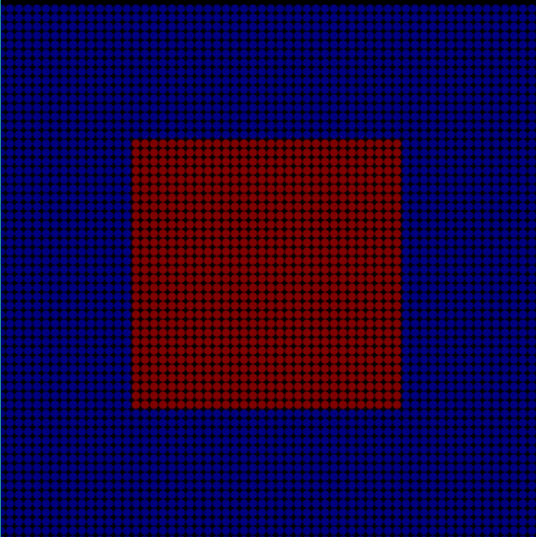
\includegraphics[trim = {1cm 1cm 1cm 1cm}, clip , angle=0, scale=0.3]{figuras/sucesso_!}
			\caption{Initial conditions.}
		\end{figure}
	\end{minipage}
	\begin{minipage}[h!]{0.30\textwidth}
		\begin{figure}[h!]
			\centering
			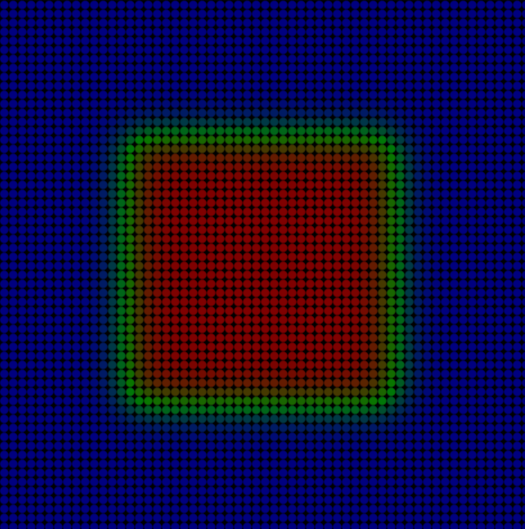
\includegraphics[trim = {1cm 1cm 1cm 1cm}, clip , angle=0, scale=0.3]{figuras/sucesso_2}
			\caption{Mid simulation.}
		\end{figure}
	\end{minipage}
	\begin{minipage}[h!]{0.30\textwidth}
		\begin{figure}[h!]
			\centering
			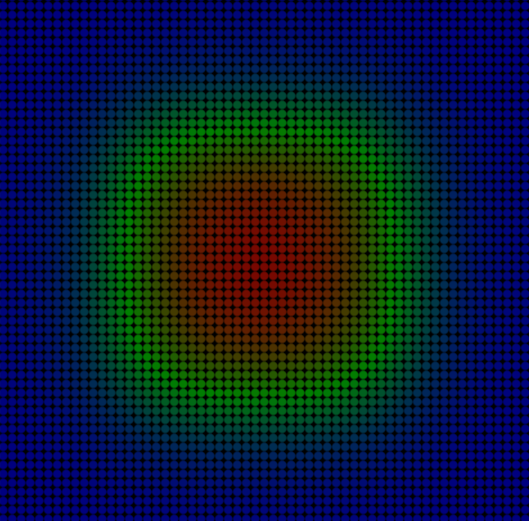
\includegraphics[trim = {1cm 1cm 1cm 1cm}, clip , angle=0, scale=0.3]{figuras/sucesso_3}
			\caption{Final time step.}
		\end{figure}
	\end{minipage}
\end{frame}

\begin{frame}
	\frametitle{Initial results}
	$\bullet$ With a $5 m/s$ velocity the vollowing results were obtained:\\
	\begin{minipage}[h!]{0.30\textwidth}
		\begin{figure}[h!]
			\centering
			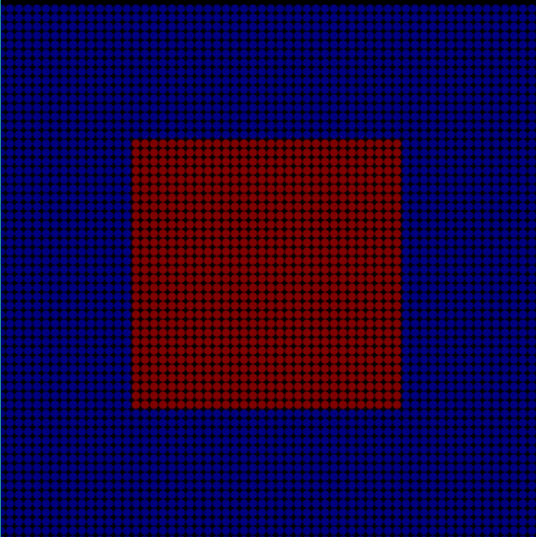
\includegraphics[trim = {1cm 1cm 1cm 1cm}, clip , angle=0, scale=0.3]{figuras/sucesso_!}
			\caption{Initial condition.}
		\end{figure}
	\end{minipage}
	\begin{minipage}[h!]{0.30\textwidth}
		\begin{figure}[h!]
			\centering
			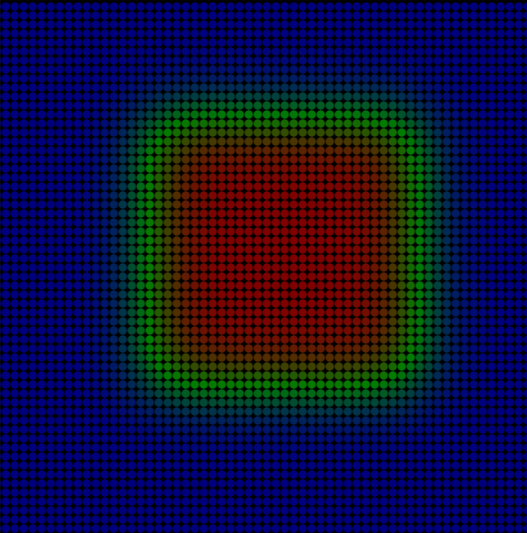
\includegraphics[trim = {1cm 1cm 1cm 1cm}, clip , angle=0, scale=0.3]{figuras/sucesso_velocidade_2}
			\caption{Mid simulation.}
		\end{figure}
	\end{minipage}
	\begin{minipage}[h!]{0.30\textwidth}
		\begin{figure}[h!]
			\centering
			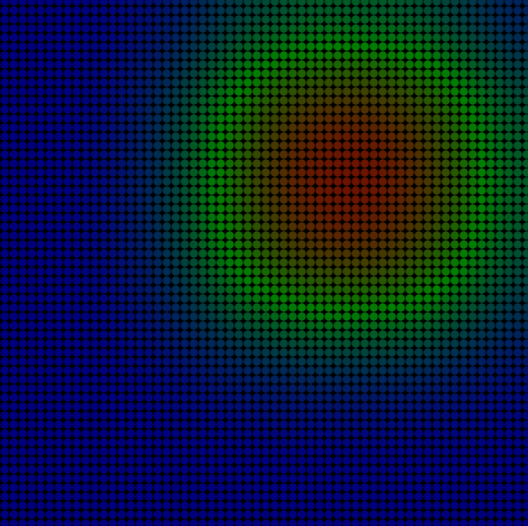
\includegraphics[trim = {1cm 1cm 1cm 1cm}, clip , angle=0, scale=0.3]{figuras/sucesso_velocidade_3}
			\caption{Last time step computed.}
		\end{figure}
	\end{minipage}
\end{frame}

\begin{frame}
	\frametitle{Error and convergence analysis}
	\begin{minipage}[h!]{0.77\textwidth}
		$\bullet$ The manufactured solution artifice was used, which consists of creating a source term and proposing a solution for t, in order to develop an exact solution for the equation when this source term is added:
		\begin{equation}
			T = e ^{1 - (x^2 + y^2 + t)}
		\end{equation}
		\begin{equation}
			G = e^{1 - (x^2 + y^2 + t)} \left( 4 \alpha - 2 u x - 2 v y - 4 \alpha (x^2 + y^2) - 1 \right)
		\end{equation}
		$\bullet$ And just like that we have the analytical solution that can be described as follows:
		\begin{equation}
			\frac{\partial T}{\partial t} + u \frac{\partial T}{\partial x} + v \frac{\partial T}{\partial y} = \alpha \left[  \frac{\partial^2 T}{\partial x^2} + \frac{\partial^2 T}{\partial y^2}   \right] + G
		\end{equation}
	\end{minipage}
	\begin{minipage}[h!]{0.17\textwidth}
		\begin{figure}[h!]
			\centering
			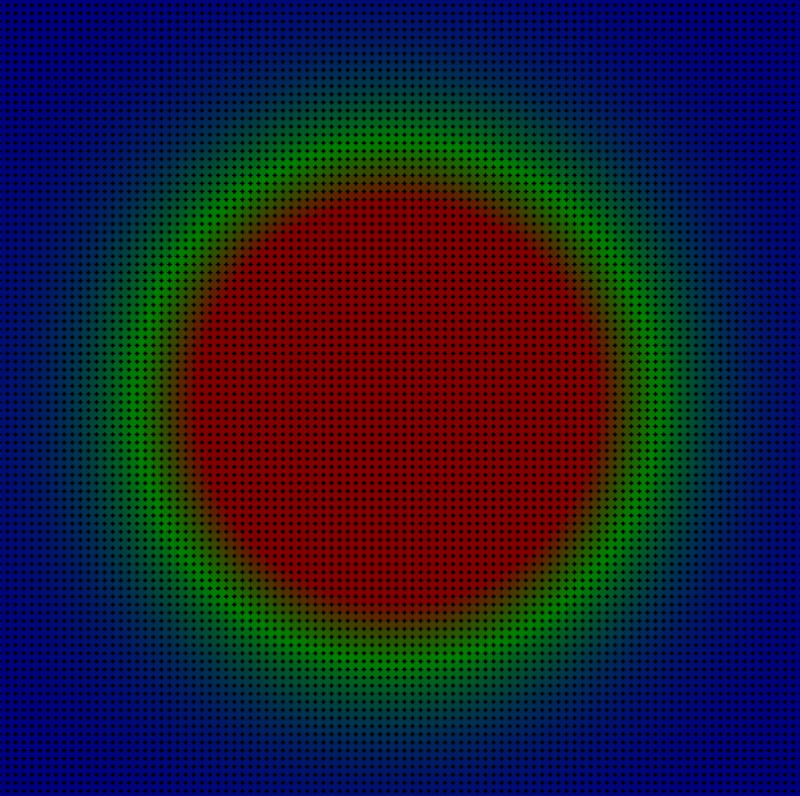
\includegraphics[trim = {0cm 0cm 0cm 0cm}, clip , angle=0, scale=0.1]{figuras/Analise_manufaturada}
			\caption{Numeric result.}
		\end{figure}
		\begin{figure}[h!]
			\centering
			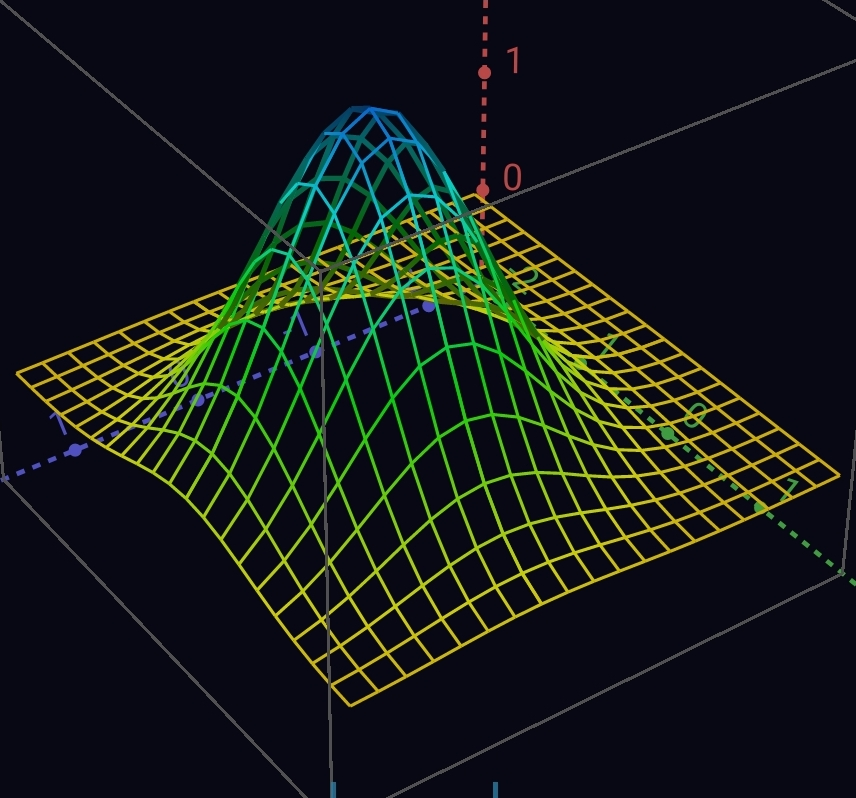
\includegraphics[trim = {0cm 0cm 0cm 0cm}, clip , angle=0, scale=0.07]{figuras/resultado_analitico}
			\caption{Analytical result.}
		\end{figure}
	\end{minipage}
\end{frame}

\begin{frame}
	\frametitle{Explicit method with source term}
	\begin{equation}
		\begin{split}
		T_{i,j}^{k} = T_{i,j}^{k-1} \left( 1 - 4 \frac{\alpha \Delta t}{\Delta s ^2}\right) + T_{i -1, j}^{k-1} \left( \alpha \frac{\Delta t}{\Delta s^2} + u \frac{\Delta t}{2 \Delta s} \right)\\
		+ T_{i,j-1}^{k-1} \left( \alpha \frac{\Delta t}{\Delta s^2} + v \frac{\Delta t}{2 \Delta s} \right) +  T_{i+1,j}^{k-1} \left( \alpha \frac{\Delta t}{ \Delta s^2} - u \frac{\Delta t}{2 \Delta s}\right) \\
		+  T_{i,j+1}^{k-1} \left( \alpha \frac{\Delta t}{\Delta s^2} - v \frac{\Delta t}{2 \Delta s}\right) + G
		\end{split}
	\end{equation}
\end{frame}

\begin{frame}
	\frametitle{Implicit method with source term}
	\begin{equation}
		\begin{split}
		T_{i,j}^{k} = \frac{T_{i,j}^{k-1} + T_{i -1, j}^{k} \left( \alpha \frac{\Delta t}{\Delta s^2} + u \frac{\Delta t}{2 \Delta s} \right) 	+ T_{i,j-1}^{k} \left( \alpha \frac{\Delta t}{\Delta s^2} + v \frac{\Delta t}{2 \Delta s} \right)}{ 1 - 4 \frac{\alpha \Delta t}{\Delta s ^2}} \\
		+ \frac{  T_{i+1,j}^{k} \left( \alpha \frac{\Delta t}{ \Delta s^2} - u \frac{\Delta t}{2 \Delta s}\right)
		+  T_{i,j+1}^{k} \left( \alpha \frac{\Delta t}{\Delta s^2} - v \frac{\Delta t}{2 \Delta s}\right) + G}{ 1 - 4 \frac{\alpha \Delta t}{\Delta s ^2}}
		\end{split}
	\end{equation}
\end{frame}

\begin{frame}
	\frametitle{Simulation results}
	$\bullet$ Then, several simulations were conducted in different cfl`s, in order to observe the error behavior, the results are as follows: \\
	\begin{minipage}[h!]{0.49\textwidth}
		\begin{figure}[h!]
			\centering
			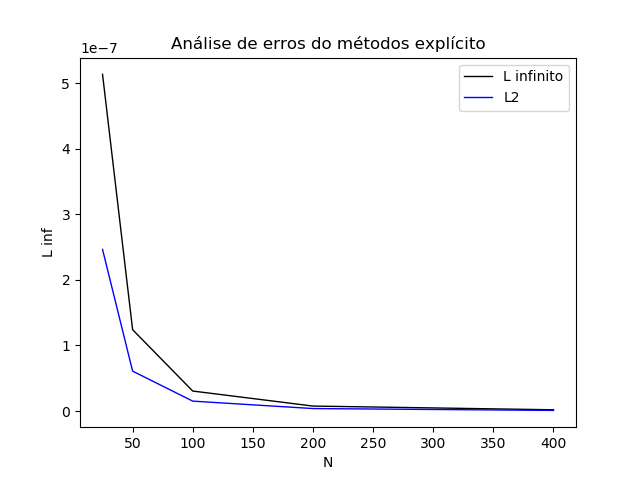
\includegraphics[trim = {0cm 0cm 0cm 0cm}, clip , angle=0, scale=0.4]{figuras/analise_de_erros_explicito}
			\caption{Convergence analysis for the explicit method. an analysis of the norms revealed a 2-order convergence. When you doubled the number of cells, it divided by approximately 4 the error.}
		\end{figure}
	\end{minipage}
	\begin{minipage}[h!]{0.49\textwidth}
		\begin{figure}[h!]
			\centering
			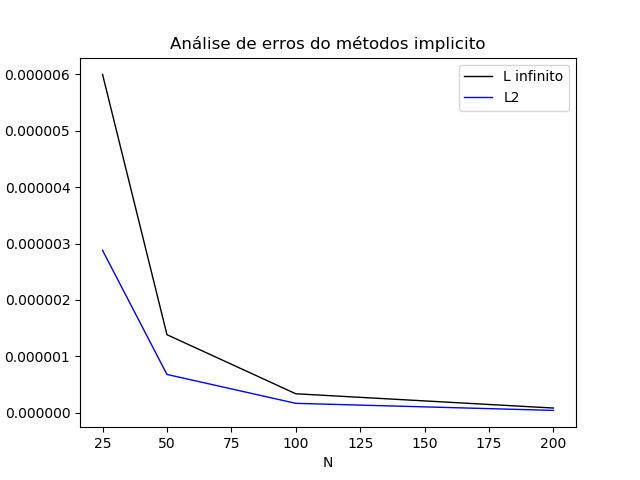
\includegraphics[trim = {0cm 0cm 0cm 0cm}, clip , angle=0, scale=0.4]{figuras/analise_de_erros_implicito}
			\caption{Convergence analysis for the implicit method. an analysis of the norms revealed a 2-order convergence. when you doubled the number of cells, it divided by approximately 4 the error.}
		\end{figure}
	\end{minipage}
\end{frame}

\begin{frame}
	\frametitle{Results}

	\begin{minipage}[h!]{0.45\textwidth}
	 	With high enough velocities some non physical results can be observed.
	\end{minipage}\hfill
 	\begin{minipage}[h!]{0.5\textwidth}
	 	\begin{figure}
	 		\animategraphics[scale = 0.25 , loop , autoplay]{10}{figuras/fortopengl/frame-}{0}{25}
	 		\label{gif_gfort}
	 		\caption{Non physical effects captured on the code.}
	 	\end{figure}
	\end{minipage}
\end{frame}

\subsection{Dynamic equations with preassure correction}

\begin{frame}
	\frametitle{Equations used}
	\flushleft
	\quad $\bullet$ Navier Stokes equation.\\
	\quad $\bullet$ Continuity.\\
	\quad $\bullet$ Energy balance equation.\\
	\quad $\bullet$ State equations.\\
	\quad $\bullet$ Boussinesq approximation.\\

	\begin{equation}
	\nabla . \vec{V} = 0
	\end{equation}
	\begin{equation}
	\frac{\partial \vec{V}}{\partial t} +  \vec{V} . {\nabla} \vec{V}  =  -\frac{1}{\rho_o} {\nabla}P + \frac{\rho - \rho_o}{\rho_o} \vec{g} + \nu \nabla ^2 \vec{V}
	\end{equation}
	\begin{equation}
	\frac{\partial T}{\partial t} + \vec{\nabla} . \left( \vec{V}T \right) = \alpha \nabla^2T
	\end{equation}
	\begin{equation}
	\frac{\rho - \rho_o}{\rho_o} = \beta \left( T - T_o\right)
	\end{equation}
\end{frame}

\begin{frame}
	\frametitle{Explicit preassure and velocity}
	\flushleft
	First, we develop the Navier Stokes equations in two forms:\vspace{0.5cm}
	\centering
	\underline{With last time step preassure domain.}
	\begin{equation}\label{equation1}
	\frac{\vec{V}^{n + 1} - \vec{V}^{n}}{\Delta t} + \vec{V}^{n} . {\nabla} \vec{V}^{n} = - \frac{1}{\rho_o}\nabla P^{n + 1} + \left( \frac{\rho - \rho_o}{\rho_o} \right) \vec{g} + \nu \nabla^2 \vec{V}^{n}
	\end{equation}
	\underline{With current time step preassure domain.}
	\begin{equation}\label{eqlabel1}
	\frac{\vec{V}^{\ast{n + 1}} - \vec{V}^{n}}{\Delta t} + \vec{V}^{n} . {\nabla} \vec{V}^{n} = - \frac{1}{\rho_o}\nabla P^{n} + \left( \frac{\rho - \rho_o}{\rho_o} \right) \vec{g} + \nu \nabla^2 \vec{V}^{n}
	\end{equation}

	Thus, subtracting the two, there is a relationship between domains:

	\begin{equation}
	\frac{\vec{V}^{{n + 1}} - \vec{V}^{{\ast n+1} }}{\Delta t} = - \frac{1}{\rho_o}\nabla \left( P^{n+1} - P ^n\right)
	\end{equation}
\end{frame}

\begin{frame}
	\frametitle{Preassure difference}
	\flushleft
	Then, we have a new variable $ P^\prime $ that describes the preassure difference between time steps.

	\begin{equation}
	P^\prime = P^{n + 1} - P^n
	\end{equation}
	Then, we have:

	\begin{equation}\label{eqlabel3}
	\vec{V}^{n+1} - \vec{V}^{\ast{n + 1}} = - \frac{\Delta t}{\rho_o} \nabla P^\prime
	\end{equation}

	Applying the diverget on both sides:

	\begin{equation}
	\nabla . \vec{V}^{n+1} - \nabla .\vec{V}^{\ast{n + 1}} = - \frac{\Delta t}{\rho_o} \nabla^2 P^\prime
	\end{equation}

	Than, form the continuity equation we have:

	\begin{equation}\label{eqlabel2}
	\nabla .\vec{V}^{\ast{n + 1}} = \frac{\Delta t}{\rho_o} \nabla^2 P^\prime
	\end{equation}
\end{frame}


\tikzstyle{rect} = [draw, rectangle,fill = red!20, text width=5em, text centered, minimum height = 2em ]
\tikzstyle{elli} = [draw, ellipse,fill=white!20,minimum height=2em]
\tikzstyle{circ} = [draw, circle,fill=white!20, minimum width=8pt,inner sep=10pt]
\tikzstyle{diam} = [draw, diamond,fill=white!20,text width=6em, text badly centered, inner sep=0pt]
\tikzstyle{line} = [draw, -latex']

\begin{frame}
	\frametitle{Data flow on each time step iteration}
	\flushleft
	So we calculate an approximated estimated velocity that we use to correct the pressure domain. 
	\begin{figure}[h]
	\begin{center}
	\begin{tikzpicture}[node distance = 1.5cm, auto]
		\node[rect, rounded corners](step1) {$\vec{V}^n $};
		\node[rect,rounded corners , right of=step1, node distance=4.5cm] (step2) {$\vec{V}^{* n + 1} $};
		\node[rect, right of=step2, node distance=6.5cm] (step3) {$P^\prime$};
		\node[rect, rounded corners, below of=step3, node distance=2.5cm](step5){$ \vec{V}^{n+1}$};

		\path[line](step1) -- node [above, text width=4em] {Explicit solution} node [below, text width=4em] {Eq.\ref{eqlabel1}} (step2);

		\path[line](step2) -- node [above, text width=4em] {Implicit solution} node (line2) [below, text width=4em] {Eq.\ref{eqlabel2}} (step3);

		\path[line](step3) -- node [right, near start,  text width=4em] {Dynamic solver} node [right, near end, text width=4em] {Eq.\ref{eqlabel3}} (step5);

		\path[line](step5) -| node [right, near end, text width=6em] {Update\\dinamic\\domain.} node [below, near start, text width=12em] {Checks continuity} (step1);
	\end{tikzpicture}
	\end{center}
	\caption{Main software iteration loop.}
	\end{figure}
\end{frame}

\begin{frame}
	\frametitle{Navier Stokes equations development}
	\centering
	\begin{equation}
		\frac{\partial \vec{V}}{\partial t} +  \vec{V} . {\nabla} \vec{V}  =  -\frac{1}{\rho_o} {\nabla}P + \frac{\rho - \rho_o}{\rho_o} \vec{g} + \nu \nabla ^2 \vec{V}
	\end{equation}
	From the vectorial equations we can separate on the three directions as follows:

	\begin{equation}
		\frac{\partial u}{\partial t} + u\frac{\partial u}{\partial x} + v\frac{\partial u}{\partial y} + w\frac{\partial u }{\partial z}  =  -\frac{1}{\rho_o} \frac{\partial P}{\partial x} + \frac{\rho - \rho_o}{\rho_o} g_x + \nu \left( \frac{\partial ^2 u}{\partial x^2} + \frac{\partial ^2 u}{\partial y^2} + \frac{\partial ^2 u}{\partial z^2} \right)
	\end{equation}

	\begin{equation}
		\frac{\partial v}{\partial t} + u\frac{\partial v}{\partial x} + v\frac{\partial v}{\partial y} + w\frac{\partial v }{\partial z}  =  -\frac{1}{\rho_o} \frac{\partial P}{\partial y} + \frac{\rho - \rho_o}{\rho_o} g_y + \nu \left( \frac{\partial ^2 v}{\partial x^2} + \frac{\partial ^2 v}{\partial y^2} + \frac{\partial ^2 v}{\partial z^2} \right)
	\end{equation}

	\begin{equation}
		\frac{\partial w}{\partial t} + u\frac{\partial w}{\partial x} + v\frac{\partial w}{\partial y} + w\frac{\partial w }{\partial z}  =  -\frac{1}{\rho_o} \frac{\partial P}{\partial z} + \frac{\rho - \rho_o}{\rho_o} g_z + \nu \left( \frac{\partial ^2 w}{\partial x^2} + \frac{\partial ^2 w}{\partial y^2} + \frac{\partial ^2 w}{\partial z^2} \right)
	\end{equation}
\end{frame}





\begin{frame}
	\frametitle{Navier Stokes equations development}
	\centering
	\begin{equation}
		\frac{\partial u}{\partial t} + u\frac{\partial u}{\partial x} + v\frac{\partial u}{\partial y} + {\color{red} w\frac{\partial u }{\partial z} } =  -\frac{1}{\rho_o} \frac{\partial P}{\partial x} + \frac{\rho - \rho_o}{\rho_o} g_x + \nu \left( \frac{\partial ^2 u}{\partial x^2} + \frac{\partial ^2 u}{\partial y^2} + { \color{red} \frac{\partial ^2 u}{\partial z^2} } \right)
	\end{equation}

	\begin{equation}
		\frac{\partial v}{\partial t} + u\frac{\partial v}{\partial x} + v\frac{\partial v}{\partial y} + {\color{red} w\frac{\partial v }{\partial z} } =  -\frac{1}{\rho_o} \frac{\partial P}{\partial y} + \frac{\rho - \rho_o}{\rho_o} g_y + \nu \left( \frac{\partial ^2 v}{\partial x^2} + \frac{\partial ^2 v}{\partial y^2} + { \color{red} \frac{\partial ^2 v}{\partial z^2} } \right)
	\end{equation}

	{\color{red}
		\begin{equation}
			\frac{\partial w}{\partial t} + u\frac{\partial w}{\partial x} + v\frac{\partial w}{\partial y} + w\frac{\partial w }{\partial z}  =  -\frac{1}{\rho_o} \frac{\partial P}{\partial z} + \frac{\rho - \rho_o}{\rho_o} g_z + \nu \left( \frac{\partial ^2 w}{\partial x^2} + \frac{\partial ^2 w}{\partial y^2} + \frac{\partial ^2 w}{\partial z^2} \right)
		\end{equation}
	}

	We can ignore the terms referent to the z dimension considering auto-similarity.
\end{frame}


\begin{frame}
	\frametitle{Explicit descrete solution}
	\centering
	\begin{equation}
		\frac{\partial u}{\partial t} + u\frac{\partial u}{\partial x} + v\frac{\partial u}{\partial y} =  -\frac{1}{\rho_o} \frac{\partial P}{\partial x} + \frac{\rho - 	\rho_o}{\rho_o} g_x + \nu \left( \frac{\partial ^2 u}{\partial x^2} + \frac{\partial ^2 u}{\partial y^2} \right)
	\end{equation}

	\begin{equation}
		\frac{\partial v}{\partial t} + u\frac{\partial v}{\partial x} + v\frac{\partial v}{\partial y} =  -\frac{1}{\rho_o} \frac{\partial P}{\partial y} + \frac{\rho - \rho_o}{\rho_o} g_y + \nu \left( \frac{\partial ^2 v}{\partial x^2} + \frac{\partial ^2 v}{\partial y^2} \right)
	\end{equation}

	Then using the Euler method for the first orther elements and central differences on the second order elements:

	\begin{equation}
		\begin{split}
		\frac{u_{i , j}^{\ast k + 1} - u_{i , j}^{k}}{\Delta t} + u_{i , j}^{k}\frac{u_{i + 1 , j}^k - u_{i - 1 , j}^k  }{2 \Delta x} + v_{i , j}^{k}\frac{u_{i , j+ 1}^k - u_{i, j-1}^k  }{2 \Delta y} =  -\frac{1}{\rho_o} \frac{P_{i, j}^k - P_{i - 1, j}^k}{\Delta x} \\ + \frac{\rho - 	\rho_o}{\rho_o} g_x + \nu \left( \frac{u_{i+1 , j}^{k} - 2 u_{i,j}^{k} + u_{i-1,j}^{k}}{\Delta x^2} + \frac{u_{i , j+1}^{k} - 2 u_{i,j}^{k} + u_{i,j-1}^{ k}}{\Delta y^2} \right)
		\end{split}
	\end{equation}
\end{frame}


\begin{frame}
	\frametitle{Explicit descrete solution}
	Thus we obtain both dynamic balance equations discretized:
	\begin{equation}
		\begin{split}
		\frac{u_{i , j}^{\ast k + 1} - u_{i , j}^{k}}{\Delta t} + u_{i , j}^{k}\frac{u_{i + 1 , j}^k - u_{i - 1 , j}^k  }{2 \Delta x} + v_{i , j}^{k}\frac{u_{i , j+ 1}^k - u_{i, j-1}^k  }{2 \Delta y} =  -\frac{1}{\rho_o} \frac{P_{i, j}^k - P_{i - 1 , j}^k}{\Delta x} \\ + \frac{\rho - 	\rho_o}{\rho_o} g_x + \nu \left( \frac{u_{i+1 , j}^{k} - 2 u_{i,j}^{k} + u_{i-1,j}^{k}}{\Delta x^2} + \frac{u_{i , j+1}^{k} - 2 u_{i,j}^{k} + u_{i,j-1}^{k}}{\Delta y^2} \right)
		\end{split}
	\end{equation}
	\begin{equation}
		\begin{split}
		\frac{v_{i , j}^{\ast k + 1} - v_{i , j}^{k}}{\Delta t} + u_{i , j}^{k}\frac{v_{i + 1 , j}^k - v_{i - 1 , j}^k  }{2 \Delta x} + v_{i , j}^{k}\frac{v_{i , j+ 1}^k - v_{i, j-1}^k  }{2 \Delta y} =  -\frac{1}{\rho_o} \frac{P_{i , j}^k - P_{i , j - 1}^k}{\Delta y} \\ + \frac{\rho - \rho_o}{\rho_o} g_y + \nu \left( \frac{v_{i+1 , j}^{k} - 2 v_{i,j}^{k} + v_{i-1,j}^{k}}{\Delta x^2} + \frac{v_{i , j+1}^{k} - 2 v_{i,j}^{k} + v_{i,j-1}^{k}}{\Delta y^2} \right)
		\end{split}
	\end{equation}
\end{frame}

\begin{frame}
	\frametitle{Explicit descrete solution}
	Isolating the temporal term we obtain the explicit method:
	\begin{equation}
		\begin{split}
		u_{i , j}^{\ast k + 1} = u_{i , j}^{k} - u_{i , j}^{k}\frac{\Delta t}{2 \Delta x} \left( u_{i + 1 , j}^k - u_{i - 1 , j}^k  \right) - v_{i , j}^{k}\frac{\Delta t }{2 \Delta y} \left(u_{i , j+ 1}^k - u_{i, j-1}^k \right)  -\frac{\Delta t}{\rho_o \Delta x} \left(P_{i, j}^k - P_{i - 1 , j}^k\right)\\ + \Delta t  g_x  \frac{\rho - \rho_o}{\rho_o} + \frac{\nu \Delta t}{\Delta x^2} \left( u_{i+1 , j}^{k} - 2 u_{i,j}^{k} + u_{i-1,j}^{k} \right) + \frac{\nu \Delta t}{\Delta y^2} \left(u_{i , j+1}^{k} - 2 u_{i,j}^{k} + u_{i,j-1}^{k}\right)
		\end{split}
	\end{equation}
	\begin{equation}
		\begin{split}
		v_{i , j}^{\ast k + 1} = v_{i , j}^{k} -u_{i , j}^{k}\frac{\Delta t}{2 \Delta x} \left(v_{i + 1 , j}^k - v_{i - 1 , j}^k\right) - v_{i , j}^{k} \frac{\Delta t}{2 \Delta y} \left(v_{i , j+ 1}^k - v_{i, j-1}^k  \right) -\frac{\Delta t}{\rho_o \Delta y} \left(P_{i , j}^k - P_{i , j - 1}^k\right) \\ + \Delta t g_y  \frac{\rho - \rho_o}{\rho_o} + \frac{\nu \Delta t}{\Delta x^2} \left( v_{i+1 , j}^{k} - 2 v_{i,j}^{k} + v_{i-1,j}^{k} \right) + \frac{\nu \Delta t}{\Delta y^2} \left( v_{i , j+1}^{k} - 2 v_{i,j}^{k} + v_{i,j-1}^{k} \right)
		\end{split}
	\end{equation}
\end{frame}

\begin{frame}
	\frametitle{Implicit descrete solution}
	\begin{equation}
		\begin{split}
		\frac{u_{i , j}^{\ast k + 1} - u_{i , j}^{k}}{\Delta t} + u_{i , j}^{k}\frac{u_{i + 1 , j}^k - u_{i - 1 , j}^k  }{2 \Delta x} + v_{i , j}^{k}\frac{u_{i , j+ 1}^k - u_{i, j-1}^k  }{2 \Delta y} =  -\frac{1}{\rho_o} \frac{P_{i, j}^k - P_{i - 1 , j}^k}{\Delta x} \\ + \frac{\rho - 	\rho_o}{\rho_o} g_x + \nu \left( \frac{u_{i+1 , j}^{\ast k + 1} - 2 u_{i,j}^{\ast k + 1} + u_{i-1,j}^{\ast k + 1}}{\Delta x^2} + \frac{u_{i , j+1}^{\ast k + 1} - 2 u_{i,j}^{\ast k + 1} + u_{i,j-1}^{\ast k + 1}}{\Delta y^2} \right)
		\end{split}
	\end{equation}
	\begin{equation}
		\begin{split}
		\frac{v_{i , j}^{\ast k + 1} - v_{i , j}^{k}}{\Delta t} + u_{i , j}^{k}\frac{v_{i + 1 , j}^k - v_{i - 1 , j}^k  }{2 \Delta x} + v_{i , j}^{k}\frac{v_{i , j+ 1}^k - v_{i, j-1}^k  }{2 \Delta y} =  -\frac{1}{\rho_o} \frac{P_{i , j}^k - P_{i , j - 1}^k}{\Delta y} \\ + \frac{\rho - \rho_o}{\rho_o} g_y + \nu \left( \frac{v_{i+1 , j}^{\ast k + 1} - 2 v_{i,j}^{\ast k + 1} + v_{i-1,j}^{\ast k + 1}}{\Delta x^2} + \frac{v_{i , j+1}^{\ast k + 1} - 2 v_{i,j}^{\ast k + 1} + v_{i,j-1}^{\ast k + 1}}{\Delta y^2} \right)
		\end{split}
	\end{equation}
\end{frame}

\begin{frame}
	\frametitle{Implicit descrete solution}
	\begin{equation}
		\begin{split}
		u_{i , j}^{\ast k + 1} = \frac{u_{i , j}^{k} \Delta x ^2 \Delta y^2}{ \Delta x ^2 \Delta y^2 + 2 \nu \Delta t(\Delta x ^2 + \Delta y^2)} - \frac{ v_{i , j}^{k} \Delta x ^2 \Delta y \Delta t}{ 2 \Delta x ^2 \Delta y^2 + 4 \nu \Delta t(\Delta x ^2 + \Delta y^2)} \left( u_{i , j+ 1}^k - u_{i, j-1}^k   \right)  \\ - \frac{u_{i , j}^{k} \Delta x \Delta y^2 \Delta t}{ 2 \Delta x ^2 \Delta y^2 + 4 \nu \Delta t(\Delta x ^2 + \Delta y^2)} \left(u_{i + 1 , j}^k - u_{i - 1 , j}^k \right) - \frac{ \Delta x \Delta y^2 \Delta t}{ \rho_o \Delta x ^2 \Delta y^2 + 2 \rho_o \nu \Delta t(\Delta x ^2 + \Delta y^2)} (P_{i, j}^k - P_{i - 1 , j}^k ) \\ + \frac{ \Delta x ^2 \Delta y^2 \Delta t (\rho -\rho_o) g_x }{ \rho_o \Delta x ^2 \Delta y^2 + 2 \rho_o \nu \Delta t(\Delta x ^2 + \Delta y^2)} + \frac{ \nu \Delta y^2 {\Delta t}}{ \Delta x ^2 \Delta y^2 + 2 \nu \Delta t(\Delta x ^2 + \Delta y^2)} \left( u_{i+1 , j}^{\ast k + 1} + u_{i-1,j}^{\ast k + 1} \right) \\ + \frac{ \nu \Delta x^2 {\Delta t}}{ \Delta x ^2 \Delta y^2 + 2 \nu \Delta t(\Delta x ^2 + \Delta y^2)} \left( u_{i , j+1}^{\ast k + 1} + u_{i,j-1}^{\ast k + 1}\right)
		\end{split}
	\end{equation}

\end{frame}

\begin{frame}
	\frametitle{Implicit descrete solution}
	\begin{equation}
		\begin{split}
		v_{i , j}^{\ast k + 1} = \frac{v_{i , j}^{k} \Delta x ^2 \Delta y^2}{ \Delta x ^2 \Delta y^2 + 2 \nu \Delta t(\Delta x ^2 + \Delta y^2)} - \frac{ v_{i , j}^{k} \Delta x ^2 \Delta y \Delta t}{ 2 \Delta x ^2 \Delta y^2 + 4 \nu \Delta t(\Delta x ^2 + \Delta y^2)} \left( v_{i , j+ 1}^k - v_{i, j-1}^k   \right)  \\ - \frac{u_{i , j}^{k} \Delta x \Delta y^2 \Delta t}{ 2 \Delta x ^2 \Delta y^2 + 4 \nu \Delta t(\Delta x ^2 + \Delta y^2)} \left(v_{i + 1 , j}^k - v_{i - 1 , j}^k \right) - \frac{ \Delta x^2 \Delta y \Delta t}{ \rho_o \Delta x ^2 \Delta y^2 + 2 \rho_o \nu \Delta t(\Delta x ^2 + \Delta y^2)} (P_{i, j}^k - P_{i , j-1}^k ) \\ + \frac{ \Delta x ^2 \Delta y^2 \Delta t (\rho -\rho_o) g_y }{ \rho_o \Delta x ^2 \Delta y^2 + 2 \rho_o \nu \Delta t(\Delta x ^2 + \Delta y^2)} + \frac{ \nu \Delta y^2 {\Delta t}}{ \Delta x ^2 \Delta y^2 + 2 \nu \Delta t(\Delta x ^2 + \Delta y^2)} \left( v_{i+1 , j}^{\ast k + 1} + v_{i-1,j}^{\ast k + 1} \right) \\ + \frac{ \nu \Delta x^2 {\Delta t}}{ \Delta x ^2 \Delta y^2 + 2 \nu \Delta t(\Delta x ^2 + \Delta y^2)} \left( v_{i , j+1}^{\ast k + 1} + v_{i,j-1}^{\ast k + 1}\right)
		\end{split}
	\end{equation}
\end{frame}

\begin{frame}
	\frametitle{Preassure correction}
	For preassure correction we have, as discussed before:
	\begin{equation}
		\nabla .\vec{V}^{\ast{n + 1}} = \frac{\Delta t}{\rho_o} \nabla^2 P^\prime
	\end{equation}
	Discretizing the equation:
	\begin{equation}
		\frac{u_{i + 1 , j}^{\ast k + 1} - u_{i , j}^{\ast k + 1}}{\Delta x} + \frac{v_{i , j + 1}^{\ast k + 1} - v_{i , j}^{\ast k + 1}}{\Delta y} = \frac{\Delta t}{\rho_o} * \left( \frac{ P^{\prime}_{i + 1, j} - 2 P^{\prime}_{i , j} + P^{\prime}_{i - 1 , j} }{\Delta x^2} + \frac{ P^{\prime}_{i, j + 1} - 2 P^{\prime}_{i , j} + P^{\prime}_{i , j- 1} }{\Delta y^2} \right)
	\end{equation}
	\begin{equation}
	\frac{\rho_o}{ \Delta t} * \frac{u_{i + 1 , j}^{\ast k + 1} - u_{i , j}^{\ast k + 1}}{\Delta x} + \frac{\rho_o}{ \Delta t} * \frac{v_{i , j + 1}^{\ast k + 1} - v_{i , j}^{\ast k + 1}}{\Delta y} =  \frac{ P^{\prime}_{i + 1, j} - 2 P^{\prime}_{i , j} + P^{\prime}_{i - 1 , j} }{\Delta x^2} + \frac{ P^{\prime}_{i, j + 1} - 2 P^{\prime}_{i , j} + P^{\prime}_{i , j- 1} }{\Delta y^2}
	\end{equation}
\end{frame}


\begin{frame}
	\frametitle{Preassure correction}
	Thus we have the final descrete equation.
	\begin{equation}
		\frac{ P^{\prime}_{i + 1, j} - 2 P^{\prime}_{i , j} + P^{\prime}_{i - 1 , j} }{\Delta x^2} + \frac{ P^{\prime}_{i, j + 1} - 2 P^{\prime}_{i , j} + P^{\prime}_{i , j- 1} }{\Delta y^2} = \frac{\rho_o}{ \Delta t \Delta x} \left(u_{i + 1 , j}^{\ast k + 1} - u_{i , j}^{\ast k + 1} \right) + \frac{\rho_o}{ \Delta t \Delta y } \left( v_{i , j + 1}^{\ast k + 1} - v_{i , j}^{\ast k + 1}\right)
	\end{equation}

	\begin{equation}
		\begin{split}
		-2 P^{\prime}_{i , j} \left(   \frac{\Delta y^2 + \Delta x^2}{\Delta x^2 \Delta y^2} \right)  = \frac{\rho_o}{ \Delta t \Delta x} \left(u_{i + 1 , j}^{\ast k + 1} - u_{i , j}^{\ast k + 1} \right) + \\ \frac{\rho_o}{ \Delta t \Delta y } \left( v_{i , j + 1}^{\ast k + 1} - v_{i , j}^{\ast k + 1}\right) - \frac{1}{\Delta y^2} \left(P^{\prime}_{i , j- 1} + P^{\prime}_{i, j + 1} \right) - \frac{1}{\Delta x^2} \left(P^{\prime}_{i + 1, j} +  P^{\prime}_{i - 1 , j}\right)
		\end{split}
	\end{equation}

	\begin{equation}
	\begin{split}
	P^{\prime}_{i , j}  = - \frac{\rho_o \Delta x \Delta y^2 }{ 2 ( \Delta y^2 + \Delta x^2) \Delta t} \left(u_{i + 1 , j}^{\ast k + 1} - u_{i , j}^{\ast k + 1} \right) + \frac{\Delta y^2}{ 2 (\Delta y^2 + \Delta x^2)} \left(P^{\prime}_{i + 1, j} +  P^{\prime}_{i - 1 , j}\right) \\ - \frac{\rho_o \Delta x^2 \Delta y }{ 2 ( \Delta y^2 + \Delta x^2) \Delta t} \left( v_{i , j + 1}^{\ast k + 1} - v_{i , j}^{\ast k + 1}\right) + \frac{\Delta x^2}{ 2 (\Delta y^2 + \Delta x^2)} \left(P^{\prime}_{i , j- 1} + P^{\prime}_{i, j + 1} \right)
	\end{split}
	\end{equation}

\end{frame}


\begin{frame}
	\frametitle{Preassure correction}
	From $p^\prime$ It's possible to obtain the correct dynamic next time step, as follows:
	\begin{equation}
		\vec{V}^{k+1}  = \vec{V}^{\ast{k + 1}} - \frac{\Delta t}{\rho_o} \nabla P^\prime
	\end{equation}

	\begin{equation}
		u^{k+1}_{i, j}  = u^{\ast k+1}_{i, j} - \frac{\Delta t}{\Delta x \rho_o} \left(  P^{\prime}_{i , ii} -   P^{\prime}_{i - 1, ii}  \right)
	\end{equation}

	\begin{equation}
	v^{k+1}_{i, j}  = v^{\ast k+1}_{i, j} - \frac{\Delta t}{\Delta y \rho_o}  \left(  P^{\prime}_{i , ii} -   P^{\prime}_{i, ii-1}    \right)
	\end{equation}

\end{frame}

\begin{frame}
	\frametitle{Divergence check}
	It's important to check the divergent regularly. As our flow is incompressible this value should be zero for all the domain. So this measure is an important error indicator.
	\begin{equation}
	\frac{u_{i + 1 , ii}^{k + 1} - u_{i, ii}^{k + 1} }{\Delta x} + \frac{v_{i , ii + 1}^{k + 1} - v_{i, ii}^{k + 1} }{\Delta y} \simeq 0
	\end{equation}
\end{frame}

\begin{frame}
	\frametitle{Final fluid simulation results}
	\begin{minipage}[h!]{0.3\textwidth}
	\begin{figure}
	 	\animategraphics[scale = 0.2 , loop , autoplay]{10}{figuras/t_result/frame-}{0}{250}
	 	\caption{Temperature result for convection simulation.}
	\end{figure}
	\end{minipage}
	\begin{minipage}[h!]{0.3\textwidth}
	\begin{figure}
	 	\animategraphics[scale = 0.2 , loop , autoplay]{10}{figuras/p_result/frame-}{0}{250}
	 	\caption{Pressure result for convection simulation.}
	\end{figure}
	\end{minipage}
	\begin{minipage}[h!]{0.3\textwidth}
	\begin{figure}
	 	\animategraphics[scale = 0.2 , loop , autoplay]{10}{figuras/div_result/frame-}{0}{250}
	 	\caption{Divergent result for convection simulation.}
	\end{figure}
	\end{minipage}
\end{frame}

\begin{frame}
	\frametitle{Final fluid simulation results}
	\begin{minipage}[h!]{0.45\textwidth}
	\begin{figure}
	 	\animategraphics[scale = 0.25 , loop , autoplay]{10}{figuras/u_result/frame-}{0}{250}
	 	\caption{Horizontal velocity result.}
	\end{figure}
	\end{minipage}
	\begin{minipage}[h!]{0.45\textwidth}
	\begin{figure}
	 	\animategraphics[scale = 0.25 , loop , autoplay]{10}{figuras/v_result/frame-}{0}{250}
	 	\caption{Vertical velocity result.}
	\end{figure}
	\end{minipage}
\end{frame}

\subsection{Artificial neural network fundamentals}

\begin{frame}
	\frametitle{Anatomy of a neural network}
	\begin{minipage}[h!]{0.45\textwidth}
		A neural network can be defined by:\\
		$\bullet$ Number of input perceptrons.\\
		$\bullet$ Number of output perceptrons.\\
		$\bullet$ Number of hidden perceptron layers.\\
		$\bullet$ Activation function of each perceptron.\\
		$\bullet$ Layers structure and composition.\\
		$\bullet$ Weights of each neuron binding.\\
	\end{minipage}
	\begin{minipage}[h!]{0.45\textwidth}
	\begin{figure}[h!]
		\centering
		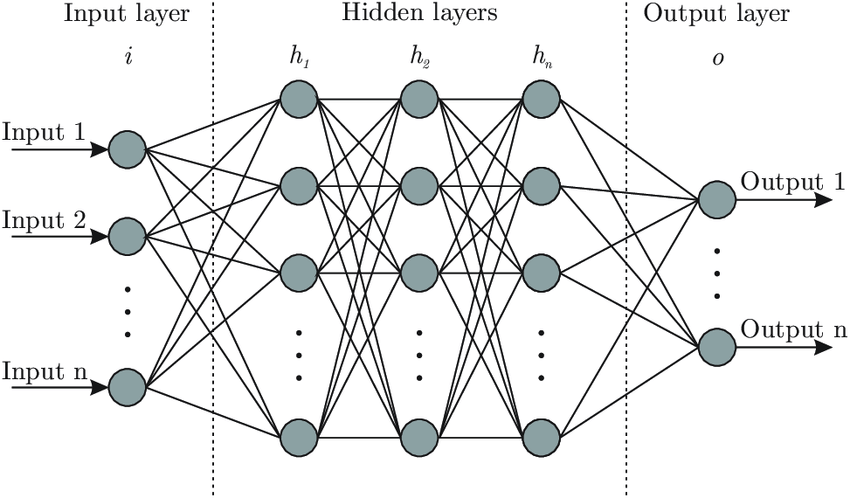
\includegraphics[trim = {0cm 0cm 0cm 0cm}, clip , angle=0, scale=0.26]{./figuras/ann_structure.png}
		\caption{Artificial neural network basic structure.}
	\end{figure}
	\end{minipage}
\end{frame}

\begin{frame}
	\frametitle{Anatomy of a neuron}
	\begin{minipage}[h!]{0.45\textwidth}
		A perceptron (or neuron) is a computational unity that defines an activation function. It stores inside itself the result of this function as demonstrated on the right.\\
		$\bullet$ $b$ is called a "bias".\\
		$\bullet$ The weight $w_i$ defines how important each relationship is. And this value, usually, is the main target of the optimization process known as "training".\\
		$\bullet$ The $x_i$ are the stored values on the input perceptrons. They can be the output of their activation functions, or the input of the entire netwok, if they are input perceptrons.\\
		$\bullet$ The $f$ value is keep inside the neuron, and becomes available for the next layer of perceptrons, or the output value of the entire network.
	\end{minipage}
	\begin{minipage}[h!]{0.45\textwidth}
	\begin{figure}[h!]
		\centering
		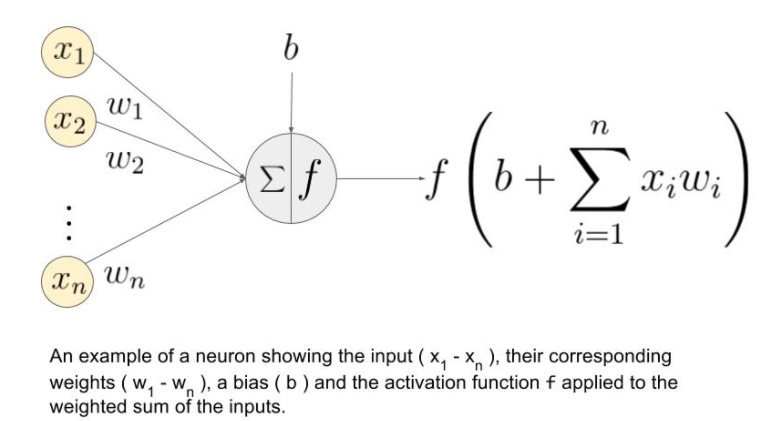
\includegraphics[trim = {0cm 3cm 11cm 0cm}, clip , angle=0, scale=0.26]{./figuras/neuron_anatomy.png}
		\caption{Perceptron anatomy.}
	\end{figure}
	\begin{equation}
		f = b + \sum^n_{i=1} x_i w_i
	\end{equation}
	\end{minipage}
\end{frame}

\begin{frame}
	\frametitle{Activation functions}
	\begin{minipage}[h!]{0.45\textwidth}
		The types of activation cab be:\ 
		$\bullet$ ReLU;\\
		$\bullet$ Hyper tangent function;\\
		$\bullet$ Identity function;\\
		$\bullet$ Binary step;\\
		$\bullet$ Logistic function or soft step;\\
		$\bullet$ Sigmoid function;\\
		$\bullet$ Arc tangent;\\
		$\bullet$ Rectified Linear Unit;\\
		$\bullet$ Exponential Linear Unit;\\
		$\bullet$ SoftPlus;\\
		$\bullet$ Gaussian;\\
		And others...

	\end{minipage}
	\begin{minipage}[h!]{0.45\textwidth}
	\begin{figure}[h!]
		\centering
		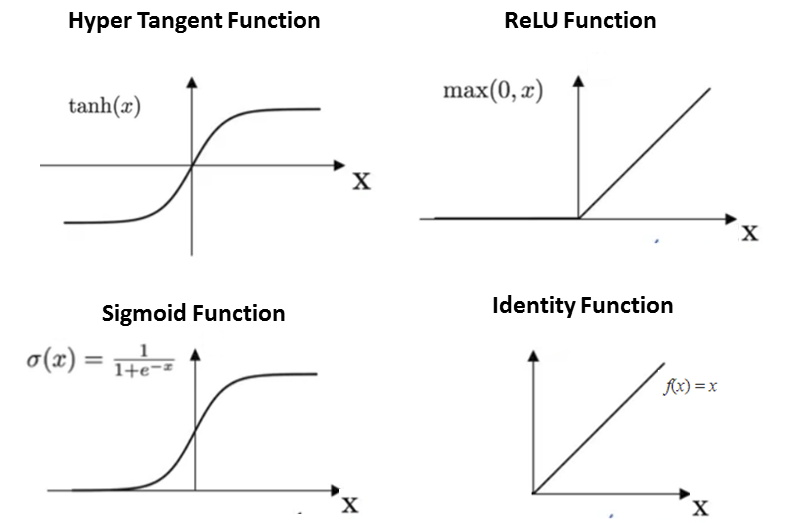
\includegraphics[trim = {0cm 0cm 0cm 0cm}, clip , angle=0, scale=0.26]{./figuras/activation_functions.png}
		\caption{Perceptron anatomy.}
	\end{figure}
	\begin{equation}
		f = b + \sum^n_{i=1} x_i w_i
	\end{equation}
	\end{minipage}
\end{frame}

\section{Acknowledgments}
	\begin{frame}
		\placelogomflab 
		\frametitle{Acknowledgments}
		\begin{figure}
		\begin{center}
		\begin{tabular}{c c}
			{
\includegraphics[trim=0.0cm 0.0cm 0.0cm 0.0cm,clip=true,height=0.2\textheight]{figuras/petrobras.png}}&{
\includegraphics[trim=0.0cm 0.0cm 0.0cm 0.0cm,clip=true,height=0.2\textheight]{figuras/logo_mflab.png}}\\
			{
\includegraphics[trim=0.0cm 0.0cm 0.0cm 0.0cm,clip=true,height=0.2\textheight]{figuras/cnpq.png}}&{
\includegraphics[trim=0.0cm 0.0cm 0.0cm 0.0cm,clip=true,height=0.2\textheight]{figuras/CAPES.png}}\\
			{
\includegraphics[trim=0.0cm 0.0cm 0.0cm 0.0cm,clip=true,height=0.2\textheight]{figuras/FAPEMIG.jpg}}&{
\includegraphics[trim=0.0cm 0.0cm 0.0cm 0.0cm,clip=true,height=0.2\textheight]{figuras/UFU_black.jpg}}\\
		\end{tabular}
		\end{center}
		\end{figure}
	\end{frame}

	\begin{frame}
		\placelogomflab 
		\frametitle{Acknowledgments}
		\fontsize{44pt}{7.2}\selectfont
		\begin{center}
			Thank you.
		\end{center}
	\end{frame}
\end{document}
